%%%%%%%%%%%%%%%%%%%%%%%%%%%%%%%%%%%%%%%%%%%%%%%%%%%%%%%%%%%%%%%%%%%%%%%%%%%%%%%%
%2345678901234567890123456789012345678901234567890123456789012345678901234567890
%        1         2         3         4         5         6         7         8
% DOCUMENT CLASS
\documentclass[oneside,12pt]{Classes/RoboticsLaTeX}

% USEFUL PACKAGES
% Commonly-used packages are included by default.
% Refer to section "Book - Useful packages" in the class file "Classes/RoboticsLaTeX.cls" for the complete list.
\usepackage{amsmath}
\usepackage{amsfonts}
\usepackage{algorithm}
\usepackage{algorithmic}
\usepackage{multirow}
\usepackage{colortbl}
\usepackage{color}
\usepackage[table]{xcolor}
\usepackage{epigraph}
\usepackage{graphicx}
%\usepackage{subfigure}
\usepackage{caption}
\usepackage{subcaption}
\usepackage{hyperref}
\usepackage{tabularx}
\usepackage{float}
\usepackage{longtable}
\usepackage[pdftex]{graphicx}
\usepackage{pdfpages}
%\usepackage{tabularx}
\usepackage{pdflscape}
\usepackage[acronym,toc]{glossaries}
\usepackage{setspace}
\usepackage[utf8]{inputenc}
\usepackage[table]{xcolor}
\usepackage{url}
\usepackage{float}
\usepackage{titlesec}
\setstretch{1.5}
%\onehalfspacing
% SPECIAL COMMANDS
% correct bad hyphenation
\hyphenation{op-tical net-works semi-conduc-tor}
\hyphenation{par-ti-cu-lar mo-du-le ge-stu-re}
% INTERLINEA 1.5
%\renewcommand{\baselinestretch}{1.5}

%% ignore slightly overfull and underfull boxes
%\hbadness=10000'
%\hfuzz=50pt
% declare commonly used operators
%\DeclareMathOperator*{\argmax}{argmax}

% HEADER
\title{\Large{Generative Adversarial Network (GAN) for Irish Traditional Music Generation}}

  \author{Tapan Vivek Auti (20231499)}
  \collegeordept{School of Computer Science}
  \university{National University of Ireland, Galway}
  \crest{
\includegraphics[width=75mm]{Figures/logo_NUI.png}}


\supervisor{Prof. Mathieu D'aquin }
%\supervisor{Name of the Supervisor}
%\supervisor{Name of the Co-Supervisor}	
% \supervisor{Dr. Jane Smith}
% \supervisorSecond{Dr. Mihael Arcan}

% text before "In partial fulfillment of the requirements for the degree of" in .cls file/line 153\
% replace PROGRAMME with Data Analytics, Artificial Intelligence, or Artificial Intelligence - Online
\degree{MSc in Computer Science (Artificial Intelligence)}
\degreedate{August 31, 2021}

%%%%%%%%%%%%%%%%%%%%%%%%%%%%%%%%%%%%%%%%%%%%%%%%%%%%%%%%%%%%%%%%%%%%%%%%%%%%%%%%
%%% uncomment if glossary needed, see examples in file
%\makeglossaries
%\loadglsentries{glossary}
\begin{document}
\begin{spacing}{1}
\maketitle
\end{spacing}
\titleformat{\chapter}[display]
  {\normalfont\huge\bfseries}{\vskip-2.5em\chaptertitlename\ \thechapter}{20pt}{\Large}
\titlespacing*{\chapter}{0pt}{*-2}{*1}


% add an empty page after title page
\newpage\null\thispagestyle{empty}\newpage

% set the number of sectioning levels that get number and appear in the contents
\setcounter{secnumdepth}{3}
\setcounter{tocdepth}{3}

\frontmatter
% replace PROGRAMME with Data Analytics, Artificial Intelligence, or Artificial Intelligence - Online
\textbf{DECLARATION} 
I, TAPAN VIVEK AUTI, do hereby declare that this thesis entitled Generative Adversarial Network (GAN) for Irish Traditional Music Generation is a bonafide record of research work done by me for the award of MSc in Computer Science (Artificial Intelligence) from National University of Ireland, Galway. It has not been previously submitted, in part or whole, to any university or institution for any degree, diploma, or other qualification. 
\newline

\begin{tabular}{@{}p{.5in}p{4in}@{}}
Signature: & ~~\hrulefill \\
\end{tabular}
\newpage


%%%% uncomment if acknowledgements needed
%\textbf{Acknowledgement}
%
%
%\newpage\textbf{}


% THESIS ABSTRACT
\begin{abstracts}

The earliest research of Neurons and other Networks can be found around 1940's and the majority of the Research that emerged over Neural Network and it's application can be evidently found after the 1980's. From then to present there have been significant changes in the applications and use of Neural Network and the concepts of Deep Learning. Many researches emerged in all fields about machines showing cognitive abilities, which is not new. The capabilities of performing human tasks and cognitive thinking  shown by machines is what debatably AI can achieve and researches in. Over the years the research gave rise to new concepts of reproducing various activities performed by human, one such being Music.

The concept of music reproduction with the help of deep learning is as well not new, but what is new is the quality of regeneration, it's similarities to original work and also the uniqueness of melodies generated. We can say the machine truly learnt and performed, along with all these things one crucial thing that is also new in today's research is the availability of resources. This thesis has tried to achieve one such similar thing where we have tried to reproduce Irish traditional folk music.

GAN model has been proposed for generation where CNN will be used as generator and as discriminator LSTM/RNN is used. ABC files have been used to train the model for music generation. The Aim of this thesis is to generate tunes that will be similar to Irish Folk Music with a model that is not specifically tuned for Irish Folk but can later be used on any type of music and generate similar tunes.

\end{abstracts}


\tableofcontents
\listoffigures
%\listoftables
\printglossary[title=List of Acronyms,type=\acronymtype]

\mainmatter

\chapter{Introduction}
\label{chap:introduction}
\section{Motivation}

The vast applications of Deep Learning in fields of computer vision, analysis, prediction, etc. are no doubt noteworthy but, the implementations and modelling used for regeneration like the one in WOMBO app for music lip syncing or Instagram filters and other similar one's have always intrigued me. The power of AI to be used to learn and reproduce something completely unique yet similar is one of the greatest researches that we have achieved over the years.

Previously having seen many applications of Deep Learning being used to reproduce melodies of various individual instruments or random noise in form of music made me realise that the scope for this and other variants are unprecedented, also having a bit of predefined interest for Folk Music we decided to use Traditional Irish Music for our thesis and to reproduce melodies that showed resemblance to the same.

The outcome we wish to achieve, were melodies generated that are not exactly sounding like one of our input songs used or like one copied from the composer directly with some minor changes, but more or less matching the same genre or theme, with the tunes being pleasant to hear and sounding like Irish Traditional Music to people hearing it for the first time. The data and model to be built on should be something which was not exactly done before with the properties of Robustness, Flexibility and Polymorphic in nature.

\section{Data Used}
For the purpose of this thesis we researched about various repositories freely available on the internet that had a clear focus on Irish Traditional Music. After thorough research we decided to go with the repository made freely available by \cite{session}.

The music files available on this site are in ABC format. Normally ABC format is converted into midi format that is then converted into .wav which we can hear as normal music. The basic ABC file looks like the following. 
\begin{verbatim}
X:1
T:Paddy O'Rafferty  
C:Trad.  
M:6/8  
K:D  
dff cee|def gfe|dff cee|dfe dBA|dff cee|def gfe|faf gfe|1 dfe dB
A:|2 dfe dcB|]  
~A3 B3|gfe fdB|AFA B2c|dfe dcB|~A3 ~B3|efe efg|faf gfe|1 dfe dcB:
2 dfe dBA|]  
fAA eAA|def gfe|fAA eAA|dfe dBA|fAA eAA|def gfe|faf gfe|dfe dBA:|
\end{verbatim}
-\cite{abcnotation}

The abc file has two parts, the header that has all the basic information including various other parameters depending on the type of file and the second part are the notes, In the example above the first five lines are the header and the last 3 lines are the notes.
\begin{verbatim}
X:1, is the reference number,
T:Paddy O'Rafferty, is the Title, 
C:Trad, defines the composer,
\end{verbatim}here it traditional as the original composer name is lost due to tune being vintage so its better to mark this as traditional, this varies according to the creator of the file.
A lot of other features are present but the ones that concern us are only X,M,K and L where M and K are the meter and key of tune, X contains the reference number that is not that important and L is note length, L being the most important as this will help us split the tune into parts if we want in preprocessing of the data.
More detailed information related to these notations and type of file is given in Chapter 2 - Background.
\section{Flow of Thesis}
\textbf{Chapter 1} - Gives a brief introduction to the thesis, a generic idea of the data being used, the motivation for the thesis and flow of thesis.

\noindent
\textbf{Chapter 2} - Background, gives thorough information about all the technologies that are being used in this thesis and tries to explain every concept used in brief, along with detailed explanation of the data being used and any other relevant  information related to the dataset.

\noindent
\textbf{Chapter 3} - Related Work, In this chapter we have tried to cover all the prominent researches from the past that match our work and tried to explain briefly about how the advancements were made over the years till now and what their approaches were.

\noindent
\textbf{Chapter 4} - Methodology, In this chapter we have tried to give a step by step and detailed information about all the steps conducted to complete the modelling of thesis and its implementation, right from the data preprocessing to the models used and the and training done to achieve results.

\chapter{Background}
\label{chap:backg}

\section{Deep Learning}
\cite{ibm} defines deep learning as "Deep learning attempts to mimic the human brain—albeit far from matching its ability—enabling systems to cluster data and make predictions with incredible accuracy."

Deep Learning is a subfield of machine learning that deals with model or algorithms that are such constructed that they mimic the structure of our brain, basically a type of Neural Network with a lot of layers of hierarchy but always not necessarily many, with each level having some sense of abstraction that deals with the huge amount of data and processes it. There are Neural Networks with just one layer too but the addition of layers helps deal with the complexity and to get better results.

The applications of Deep Learning are way beyond imagination and the future scope where we can implement it is without question substantial.

The following is the most basic and simple representation of a NN.

\begin{figure}[H]
  \centering
  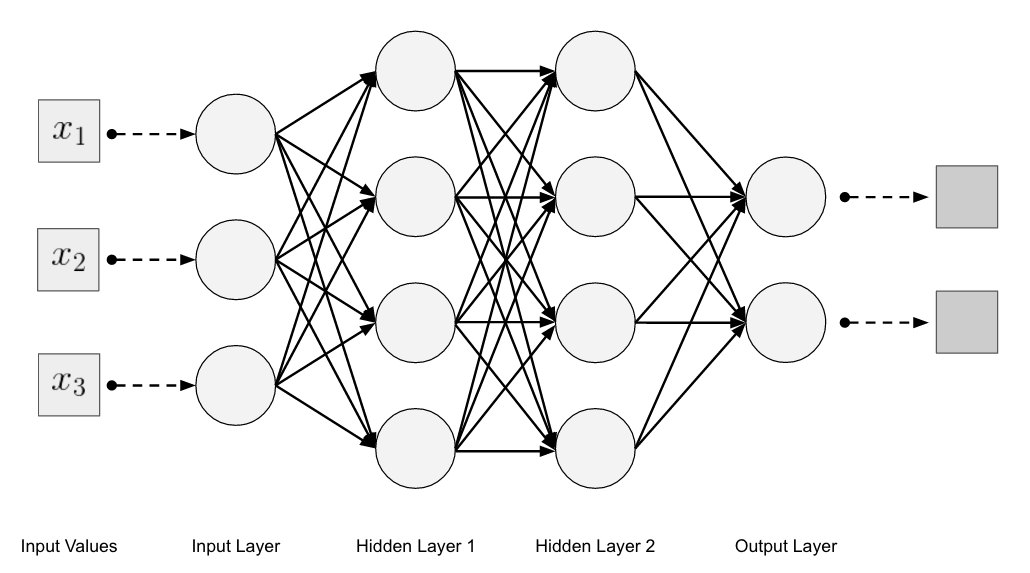
\includegraphics[width=0.80\linewidth]{Figures/dnn.png}
  \caption{Deep Neural Network}
  \label{fig:dnn}
\end{figure}

Deep Learning  uses various factors such as inputs , weights and biases that are processed upon to get accurate predictions and classifications, etc. The DNN have multiple layers and each layer has multiple nodes, these layers are built upon each other to get the most optimised solution.

\section{Recurrent Neural Network}

\cite{ibm}, "A recurrent neural network (RNN) is a type of artificial neural network which uses sequential data or time series data." Unlike Feedforward NN, RNN have their own internal memory, it uses the same function for each input and the output depends on the previous operations, the output produced is then sent back to RNN. It learns from its previous inputs and makes prediction upon them.
\begin{figure}[H]
  \centering
  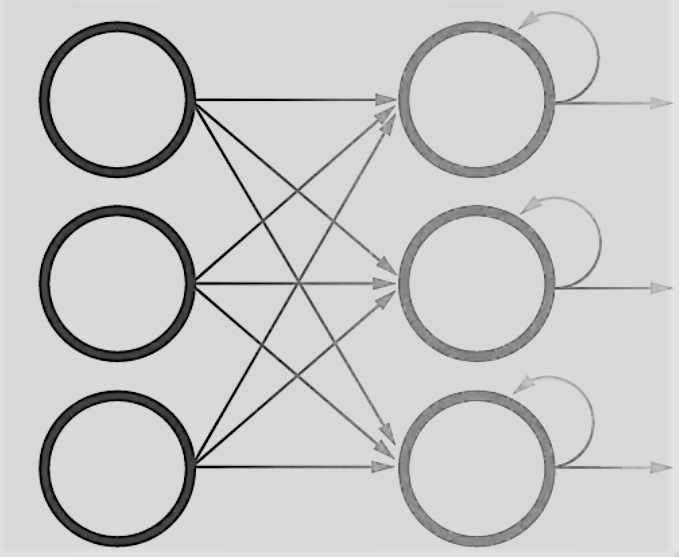
\includegraphics[width=0.5\linewidth]{Figures/rnn.png}
  \caption{Recurrent Neural Network}
  \label{fig:rnn}
\end{figure}
So basically the next step has two inputs, the output of the current state as well as the input of the state and so on. An activation function determines whether the neuron should be activated and it brings the activations to an range depending upon the functions used. The most common functions are-
\begin{itemize}
  \item Sigmoid Function:
  \begin{figure}[H]
    \centering
    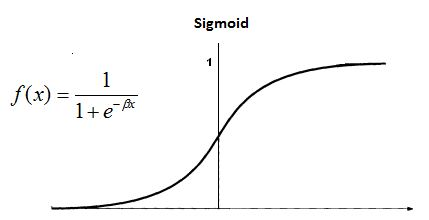
\includegraphics[width=0.5\linewidth]{Figures/sigmoid.png}
    \caption{Sigmoid Function}
    \label{fig:sigmoid}
  \end{figure}

  \item Relu Function:
  \begin{figure}[H]
    \centering
    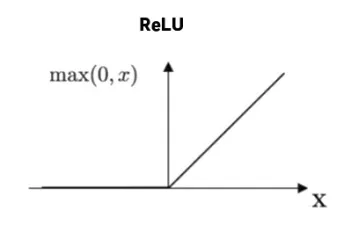
\includegraphics[width=0.5\linewidth]{Figures/relu.png}
    \caption{Relu Function}
    \label{fig:relu}
  \end{figure}

  \item Tanh Function:
  \begin{figure}[H]
    \centering
    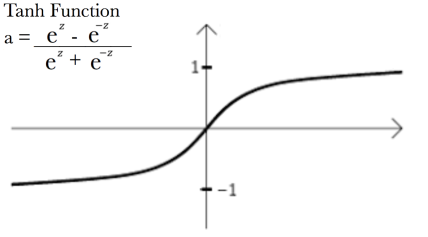
\includegraphics[width=0.5\linewidth]{Figures/tanh.png}
    \caption{Tanh Function}
    \label{fig:tanh}
  \end{figure}
\end{itemize}

\section{LSTM (Long-Term Short Memory)}
LSTM is a popular Recurrent Neural Network Architecture, it solves the problem of long-term dependencies of RNN. In cases where the current state's output is being affected by the input of states occurring much earlier in the flow, then in such case it becomes very hard for the RNN to correctly predict the output and RNN fails. To overcome this LSTM was introduced, it was first used to solve vanishing gradients problems and unlike RNN it has three states, input, output and forget gate. These control flow and give predictions.

\begin{figure}[H]
  \centering
  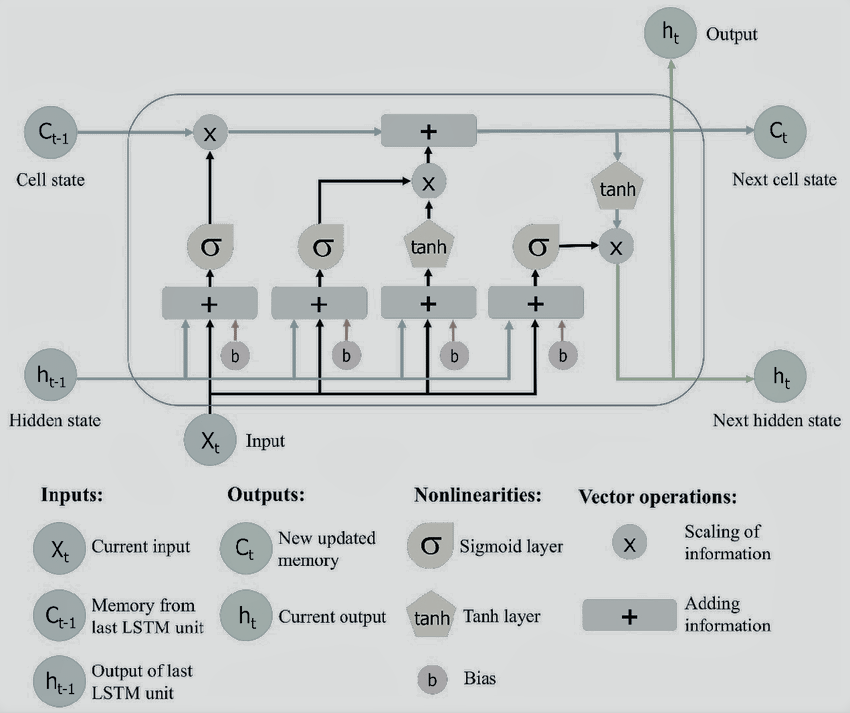
\includegraphics[width=0.90\linewidth]{Figures/lstm.png}
  \caption{LSTM Structure by \cite{yan}}
  \label{fig:lstm}
\end{figure}

\section{CNN (Convolutional Neural Network)}

Three main reasons that make CNN better than any other NN is  the convolutional layer, the pooling layer and the fully connected layer. With each layer the CNN's complexity is increased, the first few layers focus on simple features and the later on more complex identification etc. CNN have much greater performance than other with respect to image, text and audio files. The main building block of ConvNets is the convolutional layer, all the main computations occur here. It  has 3 main parts i.e. filter, feature map and the input data. \cite{ibm}

Pooling is basically a down sampling the input and deals with the dimensionality reduction of the parameters from the input. \cite{ibm} There are two main types of pooling, max pooling and average pooling.

The last Layer is the fully connected, this layer all the nodes in output layer are connected to the previous layer, this is normally the last layer of the model.

\begin{figure}[H]
  \centering
  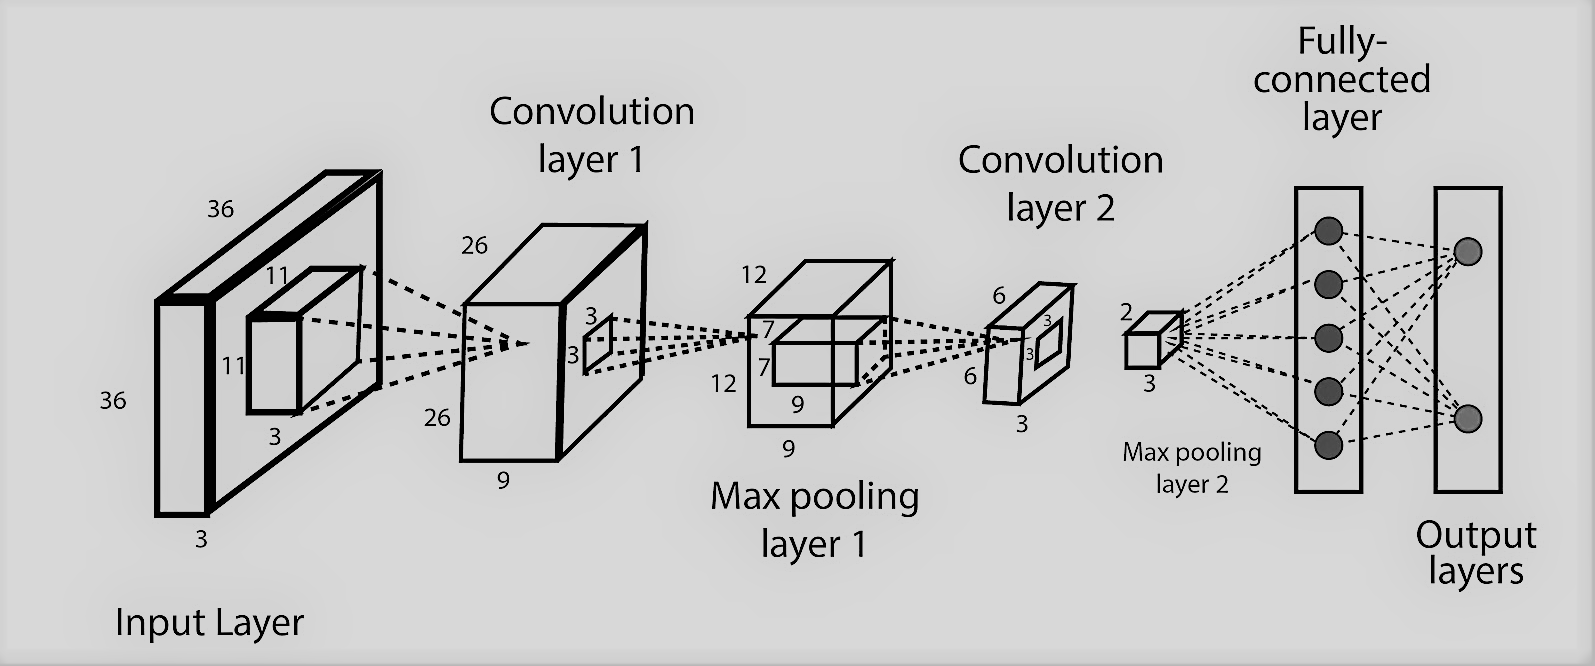
\includegraphics[width=0.90\linewidth]{Figures/cnn.png}
  \caption{ConvNets Architecture by \cite{cnnfig}}
  \label{fig:cnn}
\end{figure}

\section{GAN (Generative Adversarial Netwrok)}

This is a similar concept to that of CNN, it is a type of generative modelling,  generative modelling  is a subfield of machine learning where the features are found and learnt upon automatically from the input data in  a way that new output can be generated from the model.

There are two parts of GAN, one being the generator that creates new examples from the data and the discriminator that classifies the data, the job of the generator is to create such examples that the discriminator is not able to identify correctly and discriminator tries to find the real ones and the fake ones. The two models are run simultaneously.

\begin{figure}[H]
  \centering
  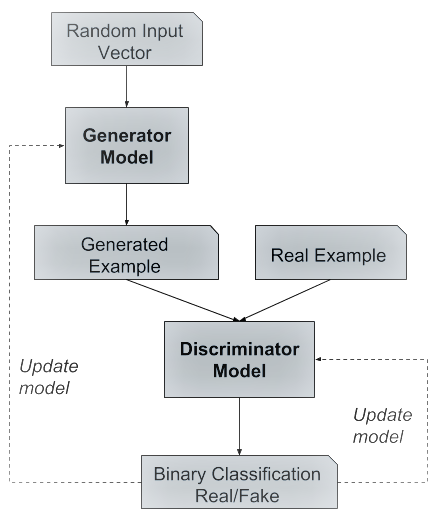
\includegraphics[width=0.5\linewidth]{Figures/gan.png}
  \caption{Architecture of GAN as defined by \cite{brownlee_2019}}
  \label{fig:gan}
\end{figure}

\section{Keras}

\cite{keras} defined "Keras is an API designed for human beings, not machines. Keras follows best practices for reducing cognitive load: it offers consistent and simple APIs, it minimizes the number of user actions required for common use cases, and it provides clear and actionable error messages. It also has extensive documentation and developer guides."

Basically Keras is a deep learning framework focusing on Neural Networks, it uses a python interface for the same, its is mostly used to deal with the various aspects of building models of NN like the layers and functions etc, it has support to CNN and RNN as well.

\section{Tensorflow}

Tensorflow is more of a open-source library with which we can perform various Machine Learning tasks.

\cite{tensorflow} defined it as "TensorFlow is an end-to-end open source platform for machine learning. It has a comprehensive, flexible ecosystem of tools, libraries and community resources that lets researchers push the state-of-the-art in ML and developers easily build and deploy ML powered applications."

It gives us the ability to build and train ML models easily, and also deploy them on cloud. It was developed by Google Brain team for internal use and used for research purposes in Google. We can debug and train keras and tensorflow code using tensorflow, it is mostly used for numerical computations using graphs.

\section{Data Representation}

The abc notations use a-g and A-G, Z for representation of notes and rests, there are other elements that denote the type of notes i.e. sharp, flat, raised or lower octave, the length and ornamentation.

High notes are depicted with " ' ", and low notes are depicted with " , " . The long notes are shown with dash or hyphen " - ". The bar line \verb+"|"+ is used to separate the bars i.e. the beat of the music.



\chapter{Related Work}
\label{chap:rel_work}

The earliest work which used Neural Network for music composition, analysis and generation can be found around late 1980's, \cite{mdolson}. This paper dealt with the traditional ways that were used for music generation, and how NN can be used to help achieve greater results, here the author used a simple implementation for music generation which used a real-time recurrent learning algorithm to generate four simple rhythms and also explained in depth about back-propagation and generalization in terms of music generation. 

What has changed from then to today, is the availability of more discrete resources for data gathering and the variations that can be found in the availability and type of data. Before, Musical data was available in non symbolic forms i.e. musical notes (polyphonic music) ,etc, it was very hard to train and was complex in training aspects due to scarce availability of data. The availability of resources has paved a new pathway for more advancements in 'deep learning', \cite{deeplearning}, and hence a lot of research has been conducted since then regarding music generation with Neural Network.

\cite{jpon} suggests that all earlier work was done using a single melody, that means only a single instrument was used or only one note was used to generate music, piano rolls were amongst the most common one's used. The majority  of the research being conducted for music generation was done using RNN and LSTM,  \cite{lstmtemporal}, \cite{rnnmelodies}, \cite{eck}.

The very first one's to use RNN was \cite{mozer}, he provided motivation for Eck and Schmidhuber, who later were the first ones to apply LSTM for music generation, \cite{eckschmid}, they thought that the music generated from RNN lacked a definite global structure and that it could not learn an entire musical form, the reason behind that being, the temporary events were not handled well by RNN and hence they thought, to deal with these issues there should be something more discrete, so they used LSTM, as RNN also had other drawbacks like failing at timing, counting and CSL learning which were removed using LSTM.

\cite{abcmusic} did the most significant use of sequential ABC files for music generation using LSTM, they in the paper suggest two models for it ,one is Char RNN, which uses a single character vocabulary and other is Folk RNN, which used transcription token for generation. They were the first one's to successfully use ABC file for music generation, they preprocessed and separated tunes based on single and transcription tokens and then passed them to the beforementioned models to obtain two different results. Till date the only type of research done on music regeneration was mostly on piano rolls which uses midi files for regeneration , \cite{midinet}, \cite{musegan}. These piano rolls generally comprise of tunes from a single instrument and rarely have tunes from multiple instruments. This made a stagnancy in type of music generated, as more or less the dataset used as input was similar. The models used differ in all papers which to give rise to variations in the music produced  but still somehow show a sense of similarity when mapped with the melody's. Very few models and papers were such that used a combination of multiple instruments and completely new models which produced unique and never before heard melodies.

\cite{polygan} and various other models were generally polyphonic music generation models, these generated polyphonic music by taking midi files as input. Till late 2018 \cite{crnngan} was the only model that used GAN for music generation, it used midi files as input, but had drawbacks of not being able to generate music using priming melody or chord sequences, these were removed in \cite{midinet}. MIDINET used CNN as their main base model which gave them better results.

After various researches it was proved that CNN is faster than RNN and also easily parallelizable, \cite{pxlcnn}, before this maximum models used RNN only. All the years of research has paved path for various genres of music generations, like \cite{edm} that tried to reproduce rhythm patterns of electronic music using GAN, it takes midi files of EDM and tried to reproduce this music which sounded like one that is produced on a professional instrument and resembled actual EDM to some extent.

Like symbolic data for generation, various studies were also conducted for music generation through non symbolic forms such as raw music files and wave forms. \cite{mp3net} was one such successful model that generated music from raw files, they used low convolutional GAN as their base model and achieved a milestone of having extremely low computational power while generation.

All the models that used GAN had one major drawback, that due to no or less temporal feature extraction the generated music didn't always sound natural and was unstable to overcome. \cite{dmbgan} proposed a new model that considered temporal features as well and had a self-attention mechanism to enable GAN and introduced a new method of switchable normalization to stabilize network training giving them very good results and music generated being stable and soothing to ear.

A lot of research is being made in music generation considering various aspects of music such as music generation based upon the genre or feel of music, one such proposed model is used in \cite{cvaegan}, here the authors took a dataset that has emotions tagged along with the song in the input files, so while producing output the model trains on basis of the feel of the music and generates music based on what genre you want like rowdy, romance, quiet, majestic etc.

\cite{gansynth} in 2019 was the most recent work that successfully synthesised audio by using wave files as input and using GAN for processing and generation, they used a specific controlled dataset for music generation and were able to achieve great speed which was claimed to be one thousand times faster generation than that of  \cite{wavenet}.

The latest research going on has been on music generation from lyrics, \cite{lstmgan} used LSTM generator and discriminator for generation, where in the dataset the lyrics are mapped to melodies, but comparatively such data is still very scarce to find and hence the result of the mapping is not melodies to lyrics, i.e. the generated music and lyrics not always correlate and sound good to hear, its very random and doesn't make any sense and generally sounds like music with a lot of noise in it and totally irrelevant to lyrics.

\chapter{Methodology}
\label{chap:methodology}

\section{Data Preprocessing}

\begin{itemize}
  \item Convert the abc file to string and join all songs into a single string file.
  \item Find all unique characters.
  \item Vectorize the text by creating two look tables - 
  \begin{itemize}
    \item The first lookup will map the letter to numbers 
    \item The second lookup will map the number to individual letters
  \end{itemize}
  \item Convert the String of unique character from the list of all characters to a Vectorized form.
  \item Use mapping to convert the vocabulary characters (string) to corresponding indices.
  \item The output should be numpy array with N elements where N is the length of input string.
\end{itemize}

\section{Implementation}

Yet to finalize
%%%%%%%%%%%%%%%%%%%%%%%%%%%%%%%%%%%%%%%%%%%%%%%%%%%%%%%%%%%%%%%%%%%%%%%%%%%%%%%%
\bibliographystyle{plainnat}                  % to give author-year style
\renewcommand{\bibname}{References}           % change default name Bibliography to References
\bibliography{references}                     % References file, references.bib
\addcontentsline{toc}{chapter}{References}    % add References to TOC


%%% uncomment if Appendix needed
%\appendix
%\chapter{Appendix-A-Title} 
%\label{chap:appendix_a}

%\chapter{Appendix-B-Title} 
%\label{chap:appendix_b}


\end{document}
